\documentclass[border={0.000000bp 0.000000bp 0.000000bp 0.000000bp}, 11pt]{standalone}
\pdfinfoomitdate=1
\pdftrailerid{}
\pdfsuppressptexinfo=1
\pdfinfo{ /Creator () /Producer () }

\usepackage{tikz}
\usepackage{xcolor}
\usetikzlibrary{shapes.misc}
\usetikzlibrary{backgrounds}

\definecolor{dotColorA}{HTML}{000000}
\definecolor{dotColorB}{HTML}{000000}
\definecolor{dotColorC}{HTML}{000000}
\definecolor{dotColorD}{HTML}{000000}
\definecolor{dotColorE}{HTML}{000000}
\definecolor{dotColorF}{HTML}{000000}
\definecolor{dotColorG}{HTML}{000000}
\definecolor{dotColorH}{HTML}{000000}
\definecolor{dotColorI}{HTML}{000000}
\definecolor{dotColorJ}{HTML}{000000}
\definecolor{dotColorK}{HTML}{000000}
\definecolor{dotColorL}{HTML}{000000}
\definecolor{dotColorM}{HTML}{000000}

\definecolor{labelBgColorA}{HTML}{FFFFFF}
\definecolor{labelBgColorB}{HTML}{FFFFFF}
\definecolor{labelBgColorC}{HTML}{FFFFFF}
\definecolor{labelBgColorD}{HTML}{FFFFFF}
\definecolor{labelBgColorE}{HTML}{FFFFFF}
\definecolor{labelBgColorF}{HTML}{FFFFFF}
\definecolor{labelBgColorG}{HTML}{FFFFFF}
\definecolor{labelBgColorH}{HTML}{FFFFFF}
\definecolor{labelBgColorI}{HTML}{FFFFFF}
\definecolor{labelBgColorJ}{HTML}{FFFFFF}
\definecolor{labelBgColorK}{HTML}{FFFFFF}
\definecolor{labelBgColorL}{HTML}{FFFFFF}
\definecolor{labelBgColorM}{HTML}{FFFFFF}

\definecolor{labelTextColorA}{HTML}{000000}
\definecolor{labelTextColorB}{HTML}{000000}
\definecolor{labelTextColorC}{HTML}{000000}
\definecolor{labelTextColorD}{HTML}{000000}
\definecolor{labelTextColorE}{HTML}{000000}
\definecolor{labelTextColorF}{HTML}{000000}
\definecolor{labelTextColorG}{HTML}{000000}
\definecolor{labelTextColorH}{HTML}{000000}
\definecolor{labelTextColorI}{HTML}{000000}
\definecolor{labelTextColorJ}{HTML}{000000}
\definecolor{labelTextColorK}{HTML}{000000}
\definecolor{labelTextColorL}{HTML}{000000}
\definecolor{labelTextColorM}{HTML}{000000}

\definecolor{linkColorA}{HTML}{000000}
\definecolor{linkColorB}{HTML}{000000}
\definecolor{linkColorC}{HTML}{000000}
\definecolor{linkColorD}{HTML}{000000}
\definecolor{linkColorE}{HTML}{000000}
\definecolor{linkColorF}{HTML}{000000}
\definecolor{linkColorG}{HTML}{000000}
\definecolor{linkColorH}{HTML}{000000}
\definecolor{linkColorI}{HTML}{000000}
\definecolor{linkColorJ}{HTML}{000000}
\definecolor{linkColorK}{HTML}{000000}
\definecolor{linkColorL}{HTML}{000000}
\definecolor{linkColorM}{HTML}{000000}

\def\textA{\textsc{amoc}}
\def\textB{\textsc{binseg}}
\def\textC{\textsc{bocpd}}
\def\textD{\textsc{bocpdms}}
\def\textE{\textsc{cpnp}}
\def\textF{\textsc{ecp}}
\def\textG{\textsc{kcpa}}
\def\textH{\textsc{pelt}}
\def\textI{\textsc{prophet}}
\def\textJ{\textsc{rbocpdms}}
\def\textK{\textsc{rfpop}}
\def\textL{\textsc{segneigh}}
\def\textM{\textsc{wbs}}

\begin{document}
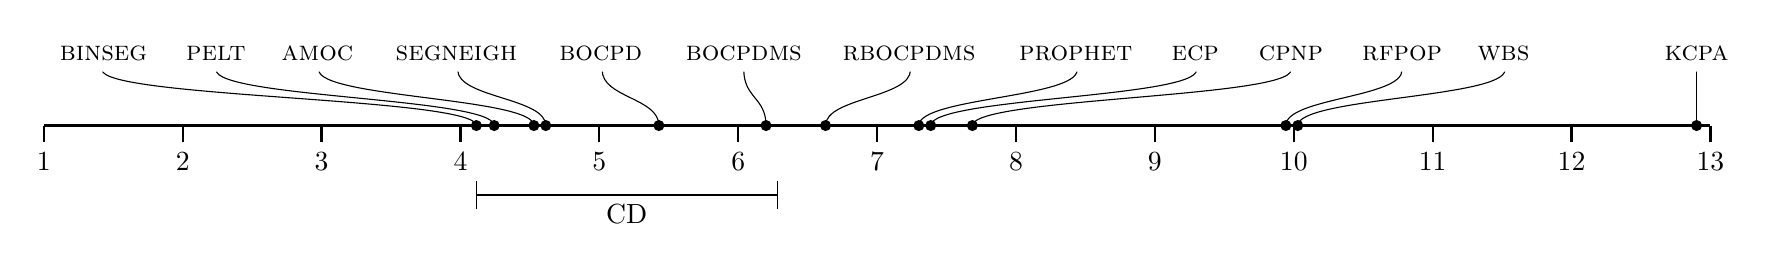
\begin{tikzpicture}[x=1bp,y=-1bp]

% shift for the margin
\begin{scope}[shift={(0, 0)}]
% main layer
\begin{scope}[shift={(0, 75)}]
% axis
\begin{scope}
\draw[very thick] (0, 0) -- (600, 0);
\end{scope}

% axis layer
\begin{scope}
\begin{scope}[shift={(0, 0)}]
\draw[thick] (0, 0) -- (0, -6pt)
node[anchor=north] {1};
\end{scope}
\begin{scope}[shift={(50, 0)}]
\draw[thick] (0, 0) -- (0, -6pt)
node[anchor=north] {2};
\end{scope}
\begin{scope}[shift={(100, 0)}]
\draw[thick] (0, 0) -- (0, -6pt)
node[anchor=north] {3};
\end{scope}
\begin{scope}[shift={(150, 0)}]
\draw[thick] (0, 0) -- (0, -6pt)
node[anchor=north] {4};
\end{scope}
\begin{scope}[shift={(200, 0)}]
\draw[thick] (0, 0) -- (0, -6pt)
node[anchor=north] {5};
\end{scope}
\begin{scope}[shift={(250, 0)}]
\draw[thick] (0, 0) -- (0, -6pt)
node[anchor=north] {6};
\end{scope}
\begin{scope}[shift={(300, 0)}]
\draw[thick] (0, 0) -- (0, -6pt)
node[anchor=north] {7};
\end{scope}
\begin{scope}[shift={(350, 0)}]
\draw[thick] (0, 0) -- (0, -6pt)
node[anchor=north] {8};
\end{scope}
\begin{scope}[shift={(400, 0)}]
\draw[thick] (0, 0) -- (0, -6pt)
node[anchor=north] {9};
\end{scope}
\begin{scope}[shift={(450, 0)}]
\draw[thick] (0, 0) -- (0, -6pt)
node[anchor=north] {10};
\end{scope}
\begin{scope}[shift={(500, 0)}]
\draw[thick] (0, 0) -- (0, -6pt)
node[anchor=north] {11};
\end{scope}
\begin{scope}[shift={(550, 0)}]
\draw[thick] (0, 0) -- (0, -6pt)
node[anchor=north] {12};
\end{scope}
\begin{scope}[shift={(600, 0)}]
\draw[thick] (0, 0) -- (0, -6pt)
node[anchor=north] {13};
\end{scope}
\end{scope}

% link layer
\begin{scope}
\draw[color=linkColorA, thin] (176.42857142857144, 0) .. controls
(176.42857142857144, -10.0) and (99.0, -10.0) .. (99.0, -20.0);
\draw[color=linkColorB, thin] (155.7142857142857, 0) .. controls
(155.7142857142857, -10.0) and (21.0, -10.0) .. (21.0, -20.0);
\draw[color=linkColorC, thin] (221.42857142857144, 0) .. controls
(221.42857142857144, -10.0) and (201.0, -10.0) .. (201.0, -20.0);
\draw[color=linkColorD, thin] (260.0, 0) .. controls
(260.0, -10.0) and (252.0, -10.0) .. (252.0, -20.0);
\draw[color=linkColorE, thin] (334.2857142857143, 0) .. controls
(334.2857142857143, -10.0) and (449.0, -10.0) .. (449.0, -20.0);
\draw[color=linkColorF, thin] (319.2857142857143, 0) .. controls
(319.2857142857143, -10.0) and (415.0, -10.0) .. (415.0, -20.0);
\draw[color=linkColorG, thin] (595.0, 0) .. controls
(595.0, -10.0) and (595.0, -10.0) .. (595.0, -20.0);
\draw[color=linkColorH, thin] (162.14285714285714, 0) .. controls
(162.14285714285714, -10.0) and (62.0, -10.0) .. (62.0, -20.0);
\draw[color=linkColorI, thin] (315.0, 0) .. controls
(315.0, -10.0) and (372.0, -10.0) .. (372.0, -20.0);
\draw[color=linkColorJ, thin] (281.42857142857144, 0) .. controls
(281.42857142857144, -10.0) and (312.0, -10.0) .. (312.0, -20.0);
\draw[color=linkColorK, thin] (447.14285714285717, 0) .. controls
(447.14285714285717, -10.0) and (489.0, -10.0) .. (489.0, -20.0);
\draw[color=linkColorL, thin] (180.7142857142857, 0) .. controls
(180.7142857142857, -10.0) and (149.0, -10.0) .. (149.0, -20.0);
\draw[color=linkColorM, thin] (451.42857142857144, 0) .. controls
(451.42857142857144, -10.0) and (526.0, -10.0) .. (526.0, -20.0);
\end{scope}

% label layer
\begin{scope}
\begin{scope}[shift={(80, -34)}]
\fill[color=labelBgColorA, rounded corners=2pt]
(0, 0) rectangle (37, 14.62708) node[midway, yshift=-.75bp, anchor=center, text=labelTextColorA] {\strut \textA};
\end{scope}
\begin{scope}[shift={(0, -34)}]
\fill[color=labelBgColorB, rounded corners=2pt]
(0, 0) rectangle (43, 14.62708) node[midway, yshift=-.75bp, anchor=center, text=labelTextColorB] {\strut \textB};
\end{scope}
\begin{scope}[shift={(180, -34)}]
\fill[color=labelBgColorC, rounded corners=2pt]
(0, 0) rectangle (41, 14.62708) node[midway, yshift=-.75bp, anchor=center, text=labelTextColorC] {\strut \textC};
\end{scope}
\begin{scope}[shift={(225, -34)}]
\fill[color=labelBgColorD, rounded corners=2pt]
(0, 0) rectangle (54, 14.62708) node[midway, yshift=-.75bp, anchor=center, text=labelTextColorD] {\strut \textD};
\end{scope}
\begin{scope}[shift={(432, -34)}]
\fill[color=labelBgColorE, rounded corners=2pt]
(0, 0) rectangle (34, 14.62708) node[midway, yshift=-.75bp, anchor=center, text=labelTextColorE] {\strut \textE};
\end{scope}
\begin{scope}[shift={(401, -34)}]
\fill[color=labelBgColorF, rounded corners=2pt]
(0, 0) rectangle (27, 14.62708) node[midway, yshift=-.75bp, anchor=center, text=labelTextColorF] {\strut \textF};
\end{scope}
\begin{scope}[shift={(578, -34)}]
\fill[color=labelBgColorG, rounded corners=2pt]
(0, 0) rectangle (34, 14.62708) node[midway, yshift=-.75bp, anchor=center, text=labelTextColorG] {\strut \textG};
\end{scope}
\begin{scope}[shift={(46, -34)}]
\fill[color=labelBgColorH, rounded corners=2pt]
(0, 0) rectangle (32, 14.62708) node[midway, yshift=-.75bp, anchor=center, text=labelTextColorH] {\strut \textH};
\end{scope}
\begin{scope}[shift={(345, -34)}]
\fill[color=labelBgColorI, rounded corners=2pt]
(0, 0) rectangle (53, 14.62708) node[midway, yshift=-.75bp, anchor=center, text=labelTextColorI] {\strut \textI};
\end{scope}
\begin{scope}[shift={(281, -34)}]
\fill[color=labelBgColorJ, rounded corners=2pt]
(0, 0) rectangle (61, 14.62708) node[midway, yshift=-.75bp, anchor=center, text=labelTextColorJ] {\strut \textJ};
\end{scope}
\begin{scope}[shift={(469, -34)}]
\fill[color=labelBgColorK, rounded corners=2pt]
(0, 0) rectangle (40, 14.62708) node[midway, yshift=-.75bp, anchor=center, text=labelTextColorK] {\strut \textK};
\end{scope}
\begin{scope}[shift={(120, -34)}]
\fill[color=labelBgColorL, rounded corners=2pt]
(0, 0) rectangle (57, 14.62708) node[midway, yshift=-.75bp, anchor=center, text=labelTextColorL] {\strut \textL};
\end{scope}
\begin{scope}[shift={(511, -34)}]
\fill[color=labelBgColorM, rounded corners=2pt]
(0, 0) rectangle (29, 14.62708) node[midway, yshift=-.75bp, anchor=center, text=labelTextColorM] {\strut \textM};
\end{scope}
\end{scope}

% dots
\begin{scope}
\draw node [circle, inner sep=0pt, minimum size=4bp, 
fill=dotColorA] at (176.428571, 0) {};
\draw node [circle, inner sep=0pt, minimum size=4bp, 
fill=dotColorB] at (155.714286, 0) {};
\draw node [circle, inner sep=0pt, minimum size=4bp, 
fill=dotColorC] at (221.428571, 0) {};
\draw node [circle, inner sep=0pt, minimum size=4bp, 
fill=dotColorD] at (260.000000, 0) {};
\draw node [circle, inner sep=0pt, minimum size=4bp, 
fill=dotColorE] at (334.285714, 0) {};
\draw node [circle, inner sep=0pt, minimum size=4bp, 
fill=dotColorF] at (319.285714, 0) {};
\draw node [circle, inner sep=0pt, minimum size=4bp, 
fill=dotColorG] at (595.000000, 0) {};
\draw node [circle, inner sep=0pt, minimum size=4bp, 
fill=dotColorH] at (162.142857, 0) {};
\draw node [circle, inner sep=0pt, minimum size=4bp, 
fill=dotColorI] at (315.000000, 0) {};
\draw node [circle, inner sep=0pt, minimum size=4bp, 
fill=dotColorJ] at (281.428571, 0) {};
\draw node [circle, inner sep=0pt, minimum size=4bp, 
fill=dotColorK] at (447.142857, 0) {};
\draw node [circle, inner sep=0pt, minimum size=4bp, 
fill=dotColorL] at (180.714286, 0) {};
\draw node [circle, inner sep=0pt, minimum size=4bp, 
fill=dotColorM] at (451.428571, 0) {};
\end{scope}

% Critical difference
\def\posBest{155.7142857142856940}
\def\posCD{263.9998861756785118}
\begin{scope}
\draw (\posBest, 30) -- (\posBest, 20);
\draw (\posBest, 25) --node[below] {CD} (\posCD, 25);
\draw (\posCD, 30) -- (\posCD, 20);
\end{scope}

\end{scope}
\end{scope}
\end{tikzpicture}
\end{document}